
\chapter{시계열 분석}

{\bf 시계열(time series)}은 시스템에서 시간에 따라 변화하는 측정값 시퀀스다. 
유명한 사례는 ``하키스틱 그래프 (hockey stick graph)''로 시간에 따른 글로벌 평균 기온을 보여준다.(\url{https://en.wikipedia.org/wiki/Hockey_stick_graph} 참조).
\index{시계열 (time series)}
\index{하키스틱 그래프 (hockey stick graph)}

이번 장에서 작업할 예제는 정치과학 연구자 Zachary M. Jones에게서 왔다. 
Zachary는 미국 대마초(마리화나)에 대한 암시장(black market)을 연구한다(\url{http://zmjones.com/marijuana}). ``담배 가격 (Price of Weed)''으로 불리는 웹사이트에서 데이터를 수집했다. 이 웹사이트는 대마초 거래장소, 가격, 품질, 수량을 참여자에게 물어 시장정보를 클라우드 소싱(crowd sourcing)했다(\url{http://www.priceofweed.com/}).
이 프로젝트의 목적은 사장에 대한 합법화(legalization)같은 정책결정 효과를 조사하는 것이다. 이 프로젝트에 매력을 발견했는데 이유는 데이터를 사용해서 중요한 정치적 질문 예를 들면, 약물정책(drug policy)같이 다루기 깨문이다.

\index{담배 가격 (Price of Weed)}
\index{대마초 (cannabis)}

이번 장에서 흥미를 찾았으면하는 희망이 있지만, 분석에 전문가적인 태도를 유지하는 중요성을 반복하는 기회가 되었으면 한다. 약물(drug)가 불법 혹은 어느 약물이 불법이 되어야 하느냐는 중요하고 어려운 공공정책질문이다; 정직하게 보고된 정확한 데이터로 우리의 결정을 통보해야 한다.

\index{윤리 (ethics)}

이번 장에서 사용되는 코드는 {\tt timeseries.py}에 있다.
코드를 다운로드하고 작업하는 것에 대한 정보는 ~\ref{code}을 참조한다.

\section{가져오기(Importing)와 정제하기(cleaning)}

Mr. Jones 사이트에서 다운로드한 데이터는 이책 저장소에 있다.
다음 코드가 데이터를 읽어 판다스 데이터프레임으로 저장한다.
\index{판다스 (pandas)}
\index{데이터프레임 (DataFrame)}

\begin{verbatim}
    transactions = pandas.read_csv('mj-clean.csv', parse_dates=[5])
\end{verbatim}

\verb"parse_dates"는 5번째 칼럼(열)값을 날짜 자료형으로 해석하고, 
넘파이(NumPy) {\tt datetime64} 객체로 전환한다.
\index{넘파이 (NumPy)}

데이터프레임에는 각각 보고된 거래건에 대한 행과 다음 칼럼(열)이 있다.

\begin{itemize}

\item city (도시): 문자열 도시 이름.

\item state (주): 알파벳 두 글자로된 미국 주명.

\item price (가격): 달러로 지불된 가격.
\index{가격 (price)}

\item amount (수량): 그램으로 구입한 수량.

\item quality (품질): 구매자가 보고한 고급, 보통, 저급 품질.

\item date (날짜): 보고날짜, 추측컨데 구매일 직후 날짜.

\item ppg: 달러 표기된 그램당 가격 (price per gram)

\item state.name: 문자열 미국 주 이름

\item lat: 도시 이름에 기반한 거래가 발생한 근사치 위도 정보.

\item lon: 거래가 발생한 근사치 위도 정보.

\end{itemize}

거래 각각은 시간에 따라 발생한 사건(event)으로, 이 데이터셋을 시계열 자료로 처리할 수 있다. 하지만, 사건이 시간에 균등하게 발생하는 것은 아니다; 각 날짜별로 보고된 거래 숫자는 0건 에서 수백건으로 다양한다. 시계열을 분석하는데 사용되는 많은 방법은 측정값이 균등하게 간격으로 되어있어야 한다. 혹은 만약 데이터가 동일 간격이라면 더 간단하다.

\index{거래 (transaction)}
\index{동일 간격 데이터 (equally spaced data)}

이 방법을 시연하기 위해서, 데이터셋을 대마초 품질을 보고한 집단으로 나눈다. 그리고 나서 그램당 일별 평균 가격을 계산해서 각 집단을 동일 가격 계열(equally spaced series)로 변환한다.

\begin{verbatim}
def GroupByQualityAndDay(transactions):
    groups = transactions.groupby('quality')
    dailies = {}
    for name, group in groups:
        dailies[name] = GroupByDay(group)        

    return dailies
\end{verbatim}

{\tt groupby}는 GroupBy 객체를 반환하는 데이터프레임 메쏘드다; for 루프에 사용되서, 집단 이름과 집단을 표현하는 데이터프레임을 반복한다.
{\tt quality}가 {\tt low}, {\tt medium}, {\tt high}이기 때문에 이 이름을 갖는 집단 세개를 얻는다.

루프는 집단을 반복하는데 {\tt GroupByDay}를 호출해서 일별 평균 가격을 계산하고, 새로운 데이터프레임을 반환한다.

\begin{verbatim}
def GroupByDay(transactions, func=np.mean):
    grouped = transactions[['date', 'ppg']].groupby('date')
    daily = grouped.aggregate(func)

    daily['date'] = daily.index
    start = daily.date[0]
    one_year = np.timedelta64(1, 'Y')
    daily['years'] = (daily.date - start) / one_year

    return daily
\end{verbatim}

모수 {\tt transactions}은 데이터프레임으로 {\tt date}와 {\tt ppg}칼럼을 포함하는 데이터프레임이다. 칼럼을 두개 선택하고 나서, {\tt date} 별로 묶는다.
\index{groupby}

{\tt grouped} 결과는 날짜별로 데이터프레임으로 매핑하는데, 그 날짜에 보고된 가격을 담고 있다. {\tt aggregate}는 GroupBy 메쏘드로 집단을 반복하고, 함수를 집단 각 칼럼에 적용한다; 이 경우 칼럼은 {\tt ppg} 하나다.
그래서 {\tt aggregate} 결과는 각 날짜에 대해 행 하나와 한 칼럼 {\tt ppg}을 갖는 데이터프레임이다.
\index{aggregate}

데이터프레임에 날짜는 넘파이(NumPy) {\tt datetime64} 객체로 저장되어 있는데 10억분의 1초(nanoseconds) 64-비트 정수로 표현된다.
다음 분석을 위해서, 년도처럼 사람이 읽기 쉬운 단위로 시간 정보를 작업하는 것이 편리할 것이다. 그래서, {\tt GroupByDay}는 {\tt index}를 복사해서 {\tt date}라는 칼럼을 추가하고 나서, {\tt years}를 추가하는데 부동소수점 형식으로 첫 거래 이후로 년도 숫자를 담고 있다.
\index{넘파이 (NumPy)}
\index{datetime64}

최종결과 데이터프레임에는 {\tt ppg}, {\tt date}, {\tt years} 칼럼이 있다.
\index{데이터프레임 (DataFrame)}


\section{플롯 그리기 (Plotting)}

{\tt GroupByQualityAndDay} 결과는 각 대마초 품질로부터 일별 가격 데이터프레임으로 매핑이다. 다음에 시계열 세개를 플롯으로 그리는 코드가 있다.
\index{데이터프레임 (DataFrame)}
\index{시각화 (visualization)}

\begin{verbatim}
    thinkplot.PrePlot(rows=3)
    for i, (name, daily) in enumerate(dailies.items()):
        thinkplot.SubPlot(i+1)
        title = 'price per gram ($)' if i==0 else ''
        thinkplot.Config(ylim=[0, 20], title=title)
        thinkplot.Scatter(daily.index, daily.ppg, s=10, label=name)
        if i == 2: 
            pyplot.xticks(rotation=30)
        else:
            thinkplot.Config(xticks=[])
\end{verbatim}

{\tt rows=3}을 갖는 {\tt PrePlot}은 세개 하위그림(subplot)을 3행에 걸쳐 플롯을 그릴려고 한다는 것을 의미한다.
루프가 데이터프레임을 반복하면서 각각에 대해 산점도를 생성한다.
시계열 데이터를 플롯 그림으로 그릴 때 점들 사이를 선분(line segment)으로 표현하는 것이 일반적이다. 하지만, 이 경우에는 데이터 점이 많고, 가격 변동성이 크기 때문에, 선분을 추가는 것이 그다지 도움이 되지 못한다.
\index{thinkplot}

x-축에 라벨이 날짜라서, 가독성을 좋게 하려고 {\tt pyplot.xticks} 을 사용해서 ``ticks''을 30도 회전한다.

\index{pyplot}
\index{ticks}
\index{xticks}

\begin{figure}
% timeseries.py
\centerline{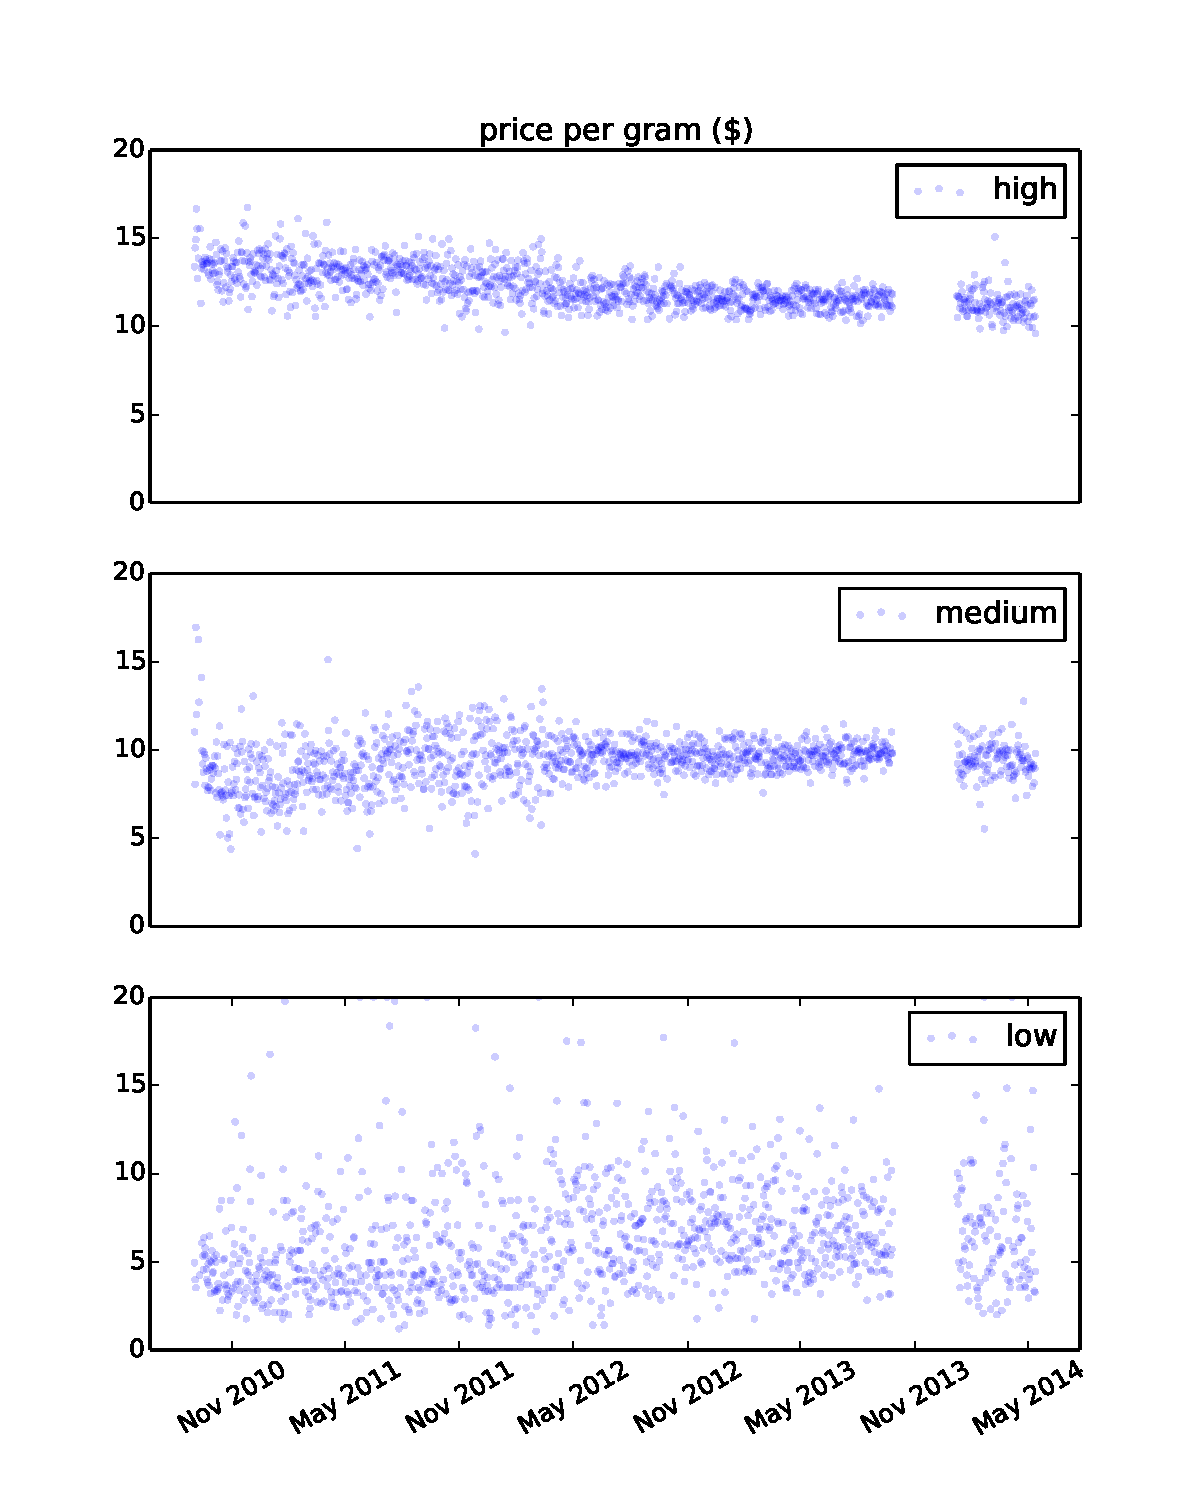
\includegraphics[width=3.5in]{figs/timeseries1.pdf}}
\caption{고급, 중급, 저급 품질 대마초에 대한 그램당 일별 시계열 그림.}
\label{timeseries1}
\end{figure}

그림~\ref{timeseries1}에 결과가 나와있다.
이 플롯 그림을 통해서 한가지 명백한 특징은 2013년 11월 틈이 있다는 것이다.
데이터 수집이 이 기간동안 활발하지 못하거나, 데이터가 이용가능하지 않았다는 것도 가능하다. 나중에 결측 데이터를 처리하는 방법을 생각해볼 것이다.
\index{결측값 (missing values)}

시각적으로 고품질 대마초 가격이 이 기간동안 하락하는 것처럼 보인다. 저품질 대마초 가격은 상승하는 것처럼 보이지만, 식별하기는 어렵다. 왜냐하면 변동성이 더 크기 때문이다. 품질 데이터는 자발적으로 보고한 것으로 시간에 따른 경향에는 참여자가 어떻게 품질 라벨을 적용했는지에 대한변동이 반영된다는 것을 기억하라.
\index{가격 (price)}


\section{선형 회귀 (Linear regression)}
\label{timeregress}

시계열분석에 특화된 방법론이 있지만, 많은 문제에 대해서, 시작하기 좋은 단순한 방법은 선형 회귀같은 범용 도구를 적용해보는 것이다.
다음 함수는 일별 가격 정보 데이터프레임을 받아서, 최소제곱 적합을 계산한다. StatsModels에서 모형과 결과 객체를 반환한다.

\index{데이터프레임 (DataFrame)}
\index{StatsModels}
\index{선형 회귀 (linear regression)}

\begin{verbatim}
def RunLinearModel(daily):
    model = smf.ols('ppg ~ years', data=daily)
    results = model.fit()
    return model, results
\end{verbatim}

그리고 나서, 수량을 반복하고 각각 모형에 적합한다.

\begin{verbatim}
    for name, daily in dailies.items():
        model, results = RunLinearModel(daily)
        print(name)
        regression.SummarizeResults(results)
\end{verbatim}

다음에 결과가 나와있다.

\begin{center}
\begin{tabular}{|l|l|l|c|} \hline
quality & intercept & slope & $R^2$ \\ \hline
high    & 13.450  & -0.708  & 0.444 \\
medium  &  8.879  & 0.283   & 0.050 \\
low     &  5.362  & 0.568   & 0.030 \\
\hline
\end{tabular}
\end{center}

추정된 기울기는 고품질 대마초 가격이 관측구간에서 매년 약 71 센트 하락했다; 중간 품질 대마초에 대해서는 매년 약 28 센트 층가했고, 저급 품질 대마초에 대해서는 매년 약 57 센트 증가했다. 이러한 추정값은 매우 작은 p-값으로 모두 통계적으로 유의하다.

\index{p-값 (p-value)}
  \index{유의성 (significant)} 
  \index{통계적 유의성 (statistically significant)}

고품질 대마초에 대한 $R^2$ 값은 0.44로 설명변수로서 시간이 관측된 가격 변동성의 44\%를 설명한다.
다른 대마초 품질에 대해서는 가격 변동이 더 작고, 가격에 변동성이 더 커서, $R^2$ 값이 더 작다(하지만, 여전히 통계적 유의성이 있다.)
\index{설명 변수 (explanatory variable)}
  \index{통계적 유의성 (statistically significant)}

다음 코드는 관측 가격과 적합값(fitted value)을 플롯으로 그린다.

\begin{verbatim}
def PlotFittedValues(model, results, label=''):
    years = model.exog[:,1]
    values = model.endog
    thinkplot.Scatter(years, values, s=15, label=label)
    thinkplot.Plot(years, results.fittedvalues, label='model')
\end{verbatim}

~\ref{implementation} 절에서 보았듯이, {\tt model}에는 {\tt exog}, {\tt endog}, 넘파이(NumPy)배열이 외생(설명), 내생(종속) 변수로 포함된다.
\index{넘파이 (NumPy)}
\index{설명변수 (explanatory variable)}
\index{종속변수 (dependent variable)}
\index{외생변수 (exogenous variable)}
\index{내생변수 (endogenous variable)}

\begin{figure}
% timeseries.py
\centerline{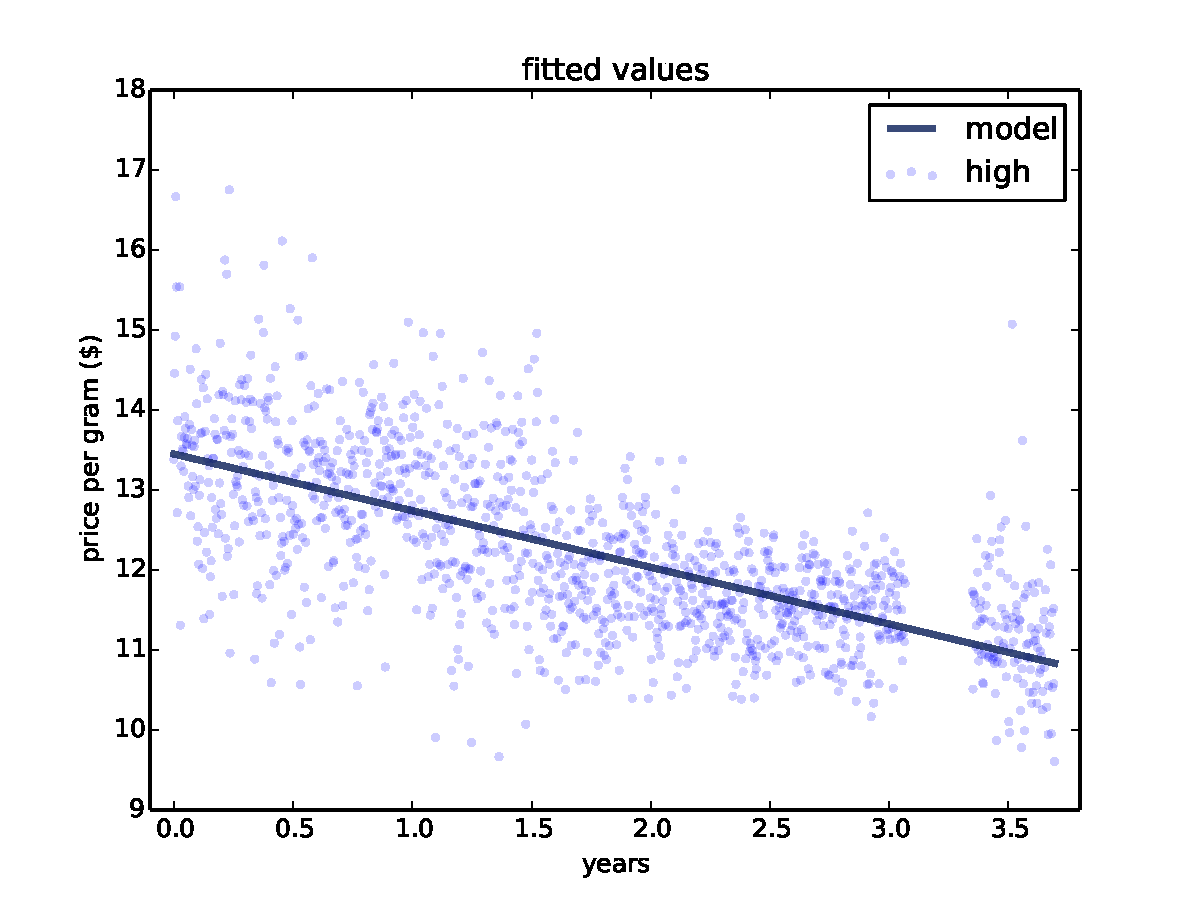
\includegraphics[height=2.5in]{figs/timeseries2.pdf}}
\caption{고급 대마초에 대한 그램당 일별가격 시계열과 선형 최소자승적합.}
\label{timeseries2}
\end{figure}

{\tt PlotFittedValues}은 데이터 점을 산점도로, 적합값을 선형 플롯 그림으로 만든다. 그림~\ref{timeseries2}에는 고품질 대마초에 대해 플롯을 그린 결과가 있다. 모형이 데이터에 대한 좋은 선형 적합처럼 보인다; 하지만, 선형회귀는 이러한 데이터에 대해서 가장 적절한 선택은 아니다.
\index{모형 (model)}
\index{적합값 (fitted values)}

\begin{itemize}

\item 첫째로, 장기 추세를 선형 혹은 다른 간단한 함수로 예측할 이유가 없다.
일반적으로, 가격은 수요와 공급에 의해 결정된다. 모두 시간에 따라 예측불가한 방향으로 변화한다.
\index{추세 (trend)}

\item 둘째, 선형회귀모형은 모든 데이터 (최근 혹은 과거)에 대해 동일한 가중치를 둔다. 예측 목적으로, 아마도 최근 데이터에 더 많은 가중치를 두어야 한다.
\index{가중치 (weight)}

\item 마지막으로, 선형회귀 가정중의 하나는 잔차가 상관되지 않는 잡음이라는 것이다. 시계열 데이터에서 연속된 값이 상관되기 때문에 종종 이런 가정은 틀리다. 
\index{잔차 (residuals)}

\end{itemize}

다음 절에서 대안을 제시하는 시계열 데이터에 대해서 더 적절하다.

\section{이동 평균 (Moving averages)}

대부분 시계열 분석은 관측된 계열이 다음 세가지 요소 합이라는 모형화 가정에 기반한다.

\index{모형 (model)}
\index{이동 평균 (moving average)}

\begin{itemize}

\item 추세 (Trend): 지속되는 변경사항을 잡아내는 평활 함수 (smooth function).
\index{추세 (trend)}

\item 계절성 (Seasonality): 주기적 변동, 아마도 일별, 주별, 월별, 혹은 년별 사이클.
\index{계절성 (seasonality)}

\item 잡음 (Noise): 장기 추세 주위 확률 변동.
\index{잡음 (noise)}

\end{itemize}

앞절에서 살펴봤듯이, 회귀는 계열에서 추세를 뽑아내는 한 방법이다. 하지만, 추세는 단순한 함수가 아니다. 훌륭한 대안은 {\bf 이동평균(moving average)}이다. 이동평균은 계열을 {\bf 윈도우(windows)}로 불리는 겹치지 않는 지역으로 나누고 각 윈도우에 있는 값을 평균낸다.
\index{윈도우 (window)}

가장 단순한 이동평균 중의 하나는 {\bf 이동평균 (rolling mean)}이다. 각 윈도우에 있는 값을 평균낸다. 예를 들어, 만약 윈도우 크기가 3이라면, 이동 평균은 0에서 2까지, 1에서 3까지, 2에서 4까지 등등 사이에 있는 값을 평균낸다.

\index{이동평균 (rolling mean)}
\index{평균 (mean)!이동 (rolling)}

판다스는에는 \verb"rolling_mean"가 있는데, 시리즈와 윈도우 크기를 인자로 받아 새로운 시리즈를 반환한다.
\index{판다스 (pandas)}
\index{시리즈 (Series)}

\begin{verbatim}
>>> series = np.arange(10)
array([0, 1, 2, 3, 4, 5, 6, 7, 8, 9])

>>> pandas.rolling_mean(series, 3)
array([ nan,  nan,   1,   2,   3,   4,   5,   6,   7,   8])
\end{verbatim}

첫 두값은 {\tt nan}이다; 다음 값은 첫 세 요소(0,1,2) 평균이다.
다음 값은 1,2,3의 평균. 등등

대마초 데이터에 \verb"rolling_mean"을 적용하기 전에, 결측값을 다루어야 한다. 하나 혹은 그 이상 대마초 품질 범주에 대해서, 관측 구간에 보고되지 않은 거래가 있는 몇일이 있고 데이터 수집이 활성화되지 않은 2013년 특정 기간이 있다.

\index{결측값 (missing values)}

지금까지 사용한 데이터프레임에 상기 날짜는 비워져있다; 인덱스는 데이터에 없는 날은 건너뛴다. 다음 분석에 대해서, 결측 데이터를 명시적으로 표기할 필요가 있다. 데이터프레임을 ``다시 인덱싱(reindexing)''해서 이 작업을 수행한다.
 \index{데이터프레임 (DataFrame)}
\index{reindex}

\begin{verbatim}
    dates = pandas.date_range(daily.index.min(), daily.index.max())
    reindexed = daily.reindex(dates)
\end{verbatim}

첫번째 행은 관측 구간 처음부터 끝까지 모든 날을 포함하는 날짜 범위를 계산한다. 두번째 행은 {\tt daily}로부터 모든 데이터를 갖는 새로운 데이터프레임을 생성하지만, {\tt nan}으로 채워진 모든 날째 행 열을 포함한다.

\index{구간 (interval)}
\index{날짜 범위 (date range)}

이제, 다음과 같이 이동평균 플롯을 그릴 수 있다.

\begin{verbatim}
    roll_mean = pandas.rolling_mean(reindexed.ppg, 30)
    thinkplot.Plot(roll_mean.index, roll_mean)
\end{verbatim}

윈도우 크기는 30이고, \verb"roll_mean"에 있는 각 값은 {\tt reindexed.ppg}으로부터 30 개값의 평균이다.

\index{판다스 (pandas)}
\index{윈도우 (window)}

\begin{figure}
% timeseries.py
\centerline{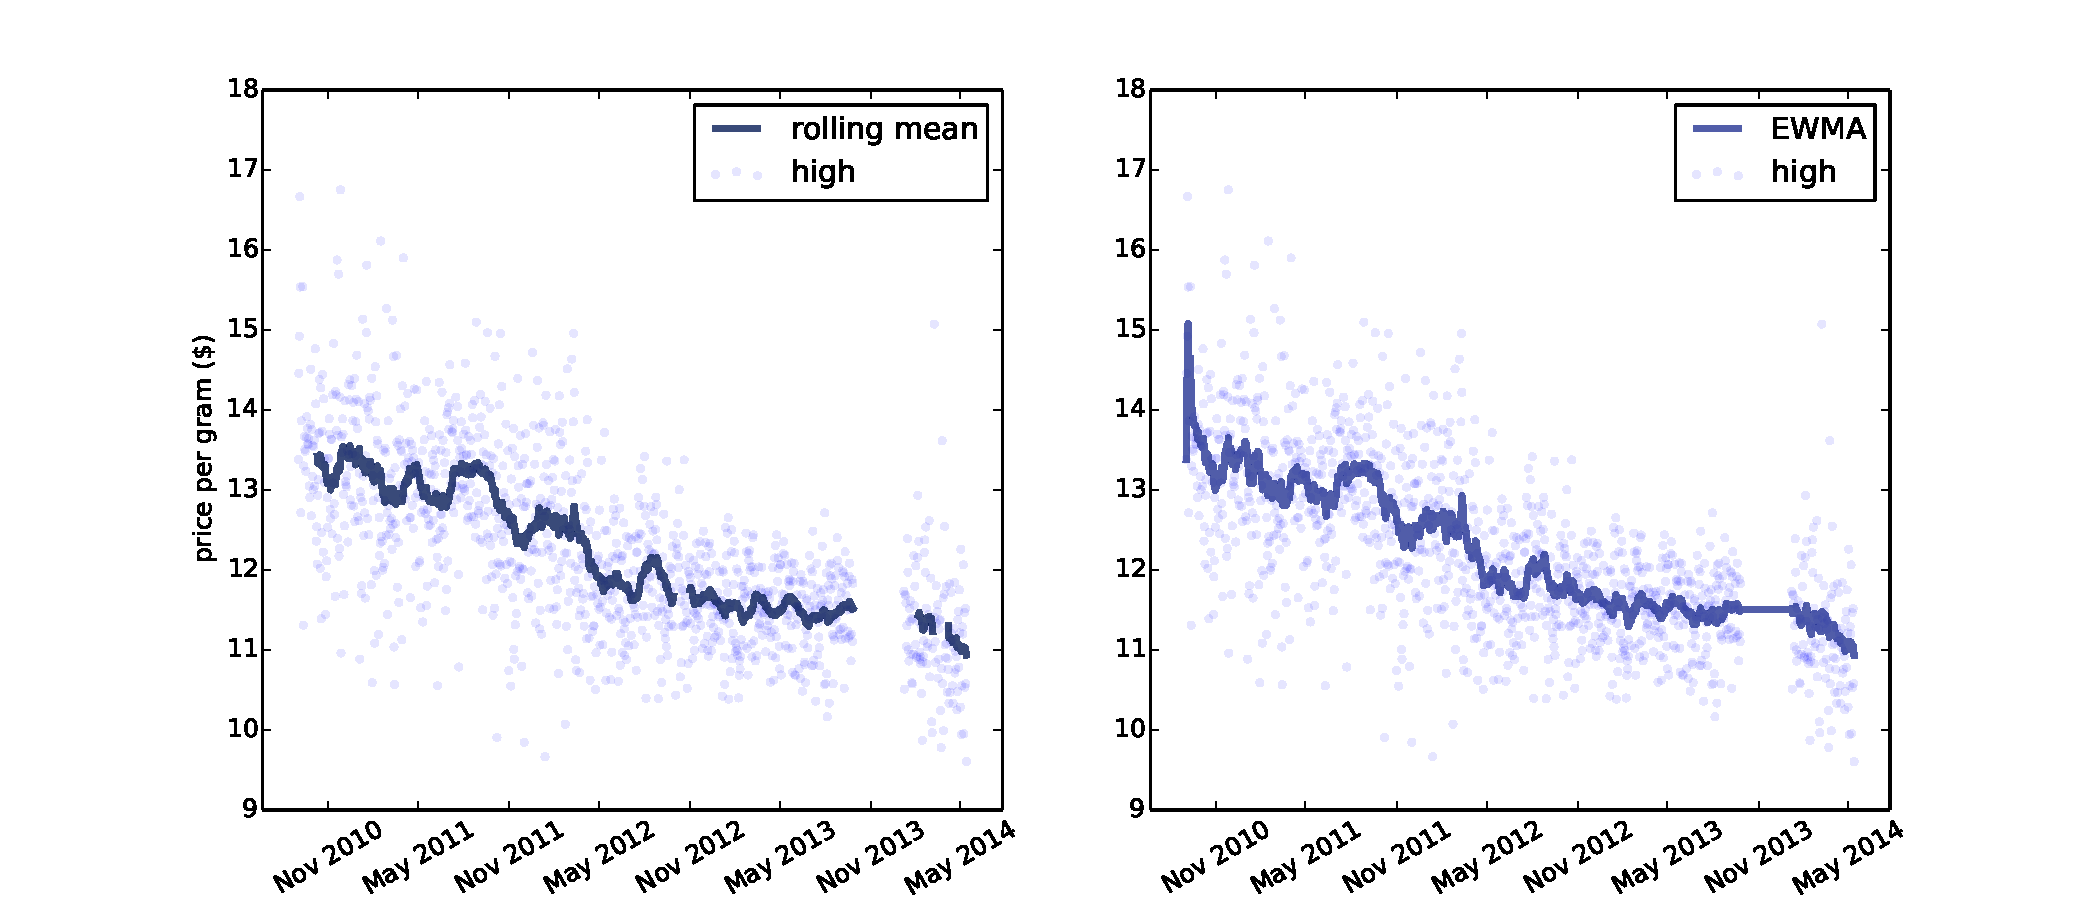
\includegraphics[height=2.5in]{figs/timeseries10.pdf}}
\caption{일별가격과 이동평균(좌측), 지수가중이동평균(exponentially-weighted moving average, EWMA, 우측).}
\label{timeseries10}
\end{figure}

그림~\ref{timeseries10} (왼편)에 결과가 그려져 있다.
이동평균은 잡음을 평활하고 추세를 추출하는 작업을 잘 하는 것처럼 보인다. 
첫 29개 값은 {\tt nan} 이고, 결측값이 있는 곳에, 또다른 {\tt nan} 29개가 다음에 있다. 이런 틈을 매울 수 있는 방법이 몇개 있지만, 성가신 작은 일이다.
\index{결측값 (missing values)}
\index{잡음 (noise)}
\index{평활 (smoothing)}

대안은 {\bf 지수가중 이동평균 (exponentially-weighted moving average)}으로 두가지 장점이 있다. 첫째, 이름에서 암시하듯이, 가중평균을 계산하는데 가장 최근 값에 가장 높은 가중치를 두고 이전 값의 가중치는 지수적으로 하락한다. 두번째, EWMA 판다스 구현이 결측값을 더 잘 처리한다.
\index{reindex}
\index{지수가중 이동평균 (exponentially-weighted moving average)}
\index{EWMA}

\begin{verbatim}
    ewma = pandas.ewma(reindexed.ppg, span=30)
    thinkplot.Plot(ewma.index, ewma)
\end{verbatim}

{\bf span} 모수는 대략 이동평균 윈도우 크기에 상응한다; 가중치가 얼마나 빨리 감쇄하는지 제어한다. 그래서 각 평균값에 무시못할 기여를 하는 점의 갯수를 결정한다.
\index{span}
\index{윈도우 (window)}

그림~\ref{timeseries10} (오른편)에 동일한 데이터에 대한 EWMA가 그려져 있다. 둘다 정의된 지점에서는 이동평균과 비슷하다. 하지만, 결측값이 없는데 작업하기 더 수월하게 한다. 시계열 시작부근에서 값들이 잡음이 있어 보이는데, 좀더 적은 데이터 점에 모형이 기반하기 때문이다.
\index{결측값 (missing values)}


\section{결측값 (Missing values)}

시계열 데이터 추세를 특성화했기 때문에, 다음 단계는 주기적인 행동인 계절성을 조사할 것이다. 인간 행동에 기반한 시계열 데이터는 종종 일별, 주별, 월별, 년별 주기(cycle)를 나타낸다. 다음 절에서, 계절성을 검정하는 방법을 제시한다. 하지만, 결측값에는 잘 동작하지 않는다. 그래서, 이 문제를 먼저 해결해야 한다.

\index{결측값 (missing values)}
\index{계절성 (seasonality)}

결측값을 채우는 간단하고 흔한 방법이 이동평균이다.
시리즈 메쏘드 {\tt fillna}가 원하는 것이다.

\index{시리즈 (Series)}
\index{fillna}

\begin{verbatim}
    reindexed.ppg.fillna(ewma, inplace=True)
\end{verbatim}

{\tt reindexed.ppg}에 {\tt nan}가 있는 곳 어디에서나, {\tt fillna}가 결측값을 {\tt ewma}에서 상응하는 값으로 교체한다. {\tt inplace} 옵션 플래그(flag)는 {\tt fillna}에 새로 생성하는 대신에 기존 시리즈를 변경하게 한다.

이 방식의 결점은 시리즈에 잡음(noise)을 과소추정하는 것이다. 재표본추출된 잔차(resampled residual)를 추가해서 이 문제를 해결할 수 있다.

\index{재표본추출 (resampling)}
\index{잡음 (noise)}

\begin{verbatim}
    resid = (reindexed.ppg - ewma).dropna()
    fake_data = ewma + thinkstats2.Resample(resid, len(reindexed))
    reindexed.ppg.fillna(fake_data, inplace=True)
\end{verbatim}

% (One note on vocabulary: in this book I am using
%``resampling'' in the statistical sense, which is drawing a random
%sample from a population that is, itself, a sample.  In the context
%of time series analysis, it has another meaning: changing the
%time between measurements in a series.  I don't use the second
%meaning in this book, but you might encounter it.)

{\tt resid}에는 {\tt ppg}가 {\tt nan}일 때 포함되지 않은 날 잔차값이 포함되어있다. \verb"fake_data"에는 이동평균 합과 잔차 확률표본(random sample)이 담겨있다. 마지막으로, {\tt fillna}는 {\tt nan}를 \verb"fake_data" 값으로 바꾼다.
\index{dropna}
\index{fillna}
\index{NaN}

\begin{figure}
% timeseries.py
\centerline{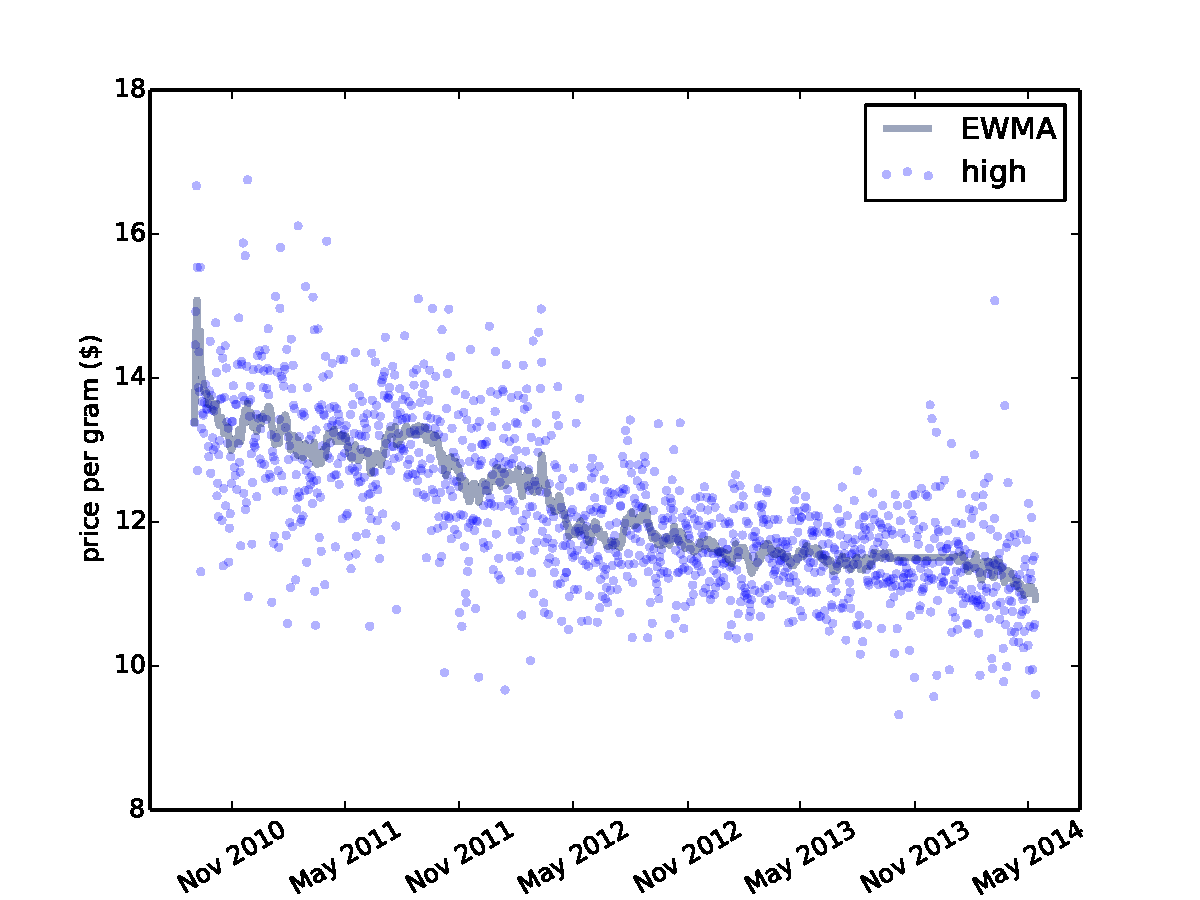
\includegraphics[height=2.5in]{figs/timeseries8.pdf}}
\caption{결측값을 채운 일별 가격.}
\label{timeseries8}
\end{figure}

그림~\ref{timeseries8}에 결과가 나와있다.
채워진 데이터는 시각적으로 실제값과 비슷하다.
재표본추출한 잔차가 랜덤(random)으로 결과는 매번 달라진다; 나중에,
결측값에서 생성된 오차를 어떻게 특성화하는지 살펴볼 것이다.

\index{재표본추출 (resampling)}
\index{결측값 (missing values)}


\section{계열 상관 (Serial correlation)}

가격은 매일 매일 변화하는데, 패턴을 보고 싶을지 모른다.
만약 월요일에 가격이 높다면, 다음 몇일동안 가격이 높을 것을 예상할 수 있다; 그리고, 만약 낮다면, 낮게 유지될 것을 예상할 수 있다.
이와 같은 패턴이 {\bf 계열 상관 (serial correlation)}이라고 부른다. 왜냐하면 각 값이 계열에 다음 값과 상관되기 때문이다.
\index{상관 (correlation)!계열 (serial)}
\index{계열 상관 (serial correlation)}

계열 상관을 계산하기 위해서, 시계열을 {\bf 시차(lag)}로 불리는 구간만큼 이동할 수 있다. 그리고 나서, 원시계열과 이동된 시계열 사이 상관을 계산한다.
\index{시차 (lag)}

\begin{verbatim}
def SerialCorr(series, lag=1):
    xs = series[lag:]
    ys = series.shift(lag)[lag:]
    corr = thinkstats2.Corr(xs, ys)
    return corr
\end{verbatim}

이동한 후에, 첫 {\tt 시차 (lag)} 값이 {\tt nan}이라, 슬라이스를 사용해서 {\tt Corr}를 계산하기 전에 제거한다.
\index{NaN}

%high 0.480121816154
%medium 0.164600078362
%low 0.103373620131

만약 {\tt SerialCorr}을 시차 1을 가진 원가격데이터에 적용하면, 계열상관이 고품질 대마초에 대해 0.48, 중간품질에는 0.16, 저품질에는 0.10이 된다.
장기 추세를 갖는 어떤 시계열에 대해서도, 강한 계열상관을 예상한다; 예를 들어, 만약 가격이 떨어지고 있다면, 계열 절반 전반부에는 평균보다 상위 값을, 계열 절반 후반부에는 평균보다 하위 값을 예상한다.

만약 추세를 제거한다면, 상관이 지속하는지 살펴보는 것이 더 흥미롭다.
예를 들어, EWMA 잔차를 계산하고 나서 계열 상관을 계산한다.
\index{EWMA}

\begin{verbatim}
    ewma = pandas.ewma(reindexed.ppg, span=30)
    resid = reindexed.ppg - ewma
    corr = SerialCorr(resid, 1)
\end{verbatim}

lag=1으로 추세 제거된 데이터에 대한 계열 상관은 고품질에는 -0.022,
중간품질에는 -0.015, 저품질에는 0.036이다.
계열 상관값이 작아서, 이 시계열 데이터에는 하루 계열상관이 매우 작거나 없다.
\index{판다스 (pandas)}

주별, 월별, 년별 계절성을 점검하기 위해서, 다시 다른 시차를 갖는 분석을 실행한다. 다음에 결과가 나와있다. 
\index{계절성 (seasonality)}

\begin{center}
\begin{tabular}{|c|c|c|c|}
\hline
lag & high & medium & low \\ \hline
1 & -0.029 & -0.014 & 0.034 \\
7 & 0.02 & -0.042 & -0.0097 \\
30 & 0.014 & -0.0064 & -0.013 \\
365 & 0.045 & 0.015 & 0.033 \\
\hline
\end{tabular}
\end{center}

다음절에서, 이러한 상관이 통계적 유의성(통계적 유의성은 없다)이 있는지 검정할 것이다. 하지만, 이 지점에서 잠정적으로 이들 시계열 데이터에 상당한 계절적 패턴이, 적어도 이런 시차에는 없다고 결론내릴 수 있다.

\index{유의성 (significant)} 
\index{통계적 유의성 (statistically significant)}


\section{자기상관 (Autocorrelation)}

만약 시계열이 계열상관을 갖고 있다고 생각하지만 어떤 시차를 검정할지 모른다면, 모든 시차를 검정할 수 있다!!! {\bf 자기상관 함수 (autocorrelation function)}는 시차에서 주어진 시차를 갖는 계열 상관에 매핑하는 함수다. ``자기상관(Autocorrelation)''은 계열상관의 또 다른 이름으로, 시차가 1이 아닐 때 더 많이 사용된다.
\index{자기상관 함수 (autocorrelation function)}

StatsModels는 ~\ref{statsmodels}절에 선형회귀에 사용했는데, 자기상관 함수를 계산하는 {\tt acf}를 포함하여 시계열분석에 함수도 제공한다.
\index{StatsModels}

\begin{verbatim}
    import statsmodels.tsa.stattools as smtsa
    acf = smtsa.acf(filled.resid, nlags=365, unbiased=True)
\end{verbatim}

{\tt acf}는 계열상관을 0 시차부터 {\tt nlags}까지 계산한다.
{\tt unbiased} 플래그옵션은 {\tt acf}에 표본크기에 대한 추정값을 보정하게 한다. 결과는 상관 배열이다. 만약 고품질 대마초에 대한 일별 가격을 선택하고, 1, 7, 30, 365 시차에 대한 상관을 추출한다면, 
{\tt acf}와 {\tt SerialCorr}는 근사적으로 거의 동일한 결과를 산출한다.
\index{acf}

\begin{verbatim}
>>> acf[0], acf[1], acf[7], acf[30], acf[365]
1.000, -0.029, 0.020, 0.014, 0.044
\end{verbatim}

{\tt lag=0}으로, {\tt acf} 본인과 계열 상관을 계산하는데, 항상 1 이다.
\index{시차 (lag)}

\begin{figure}
% timeseries.py
\centerline{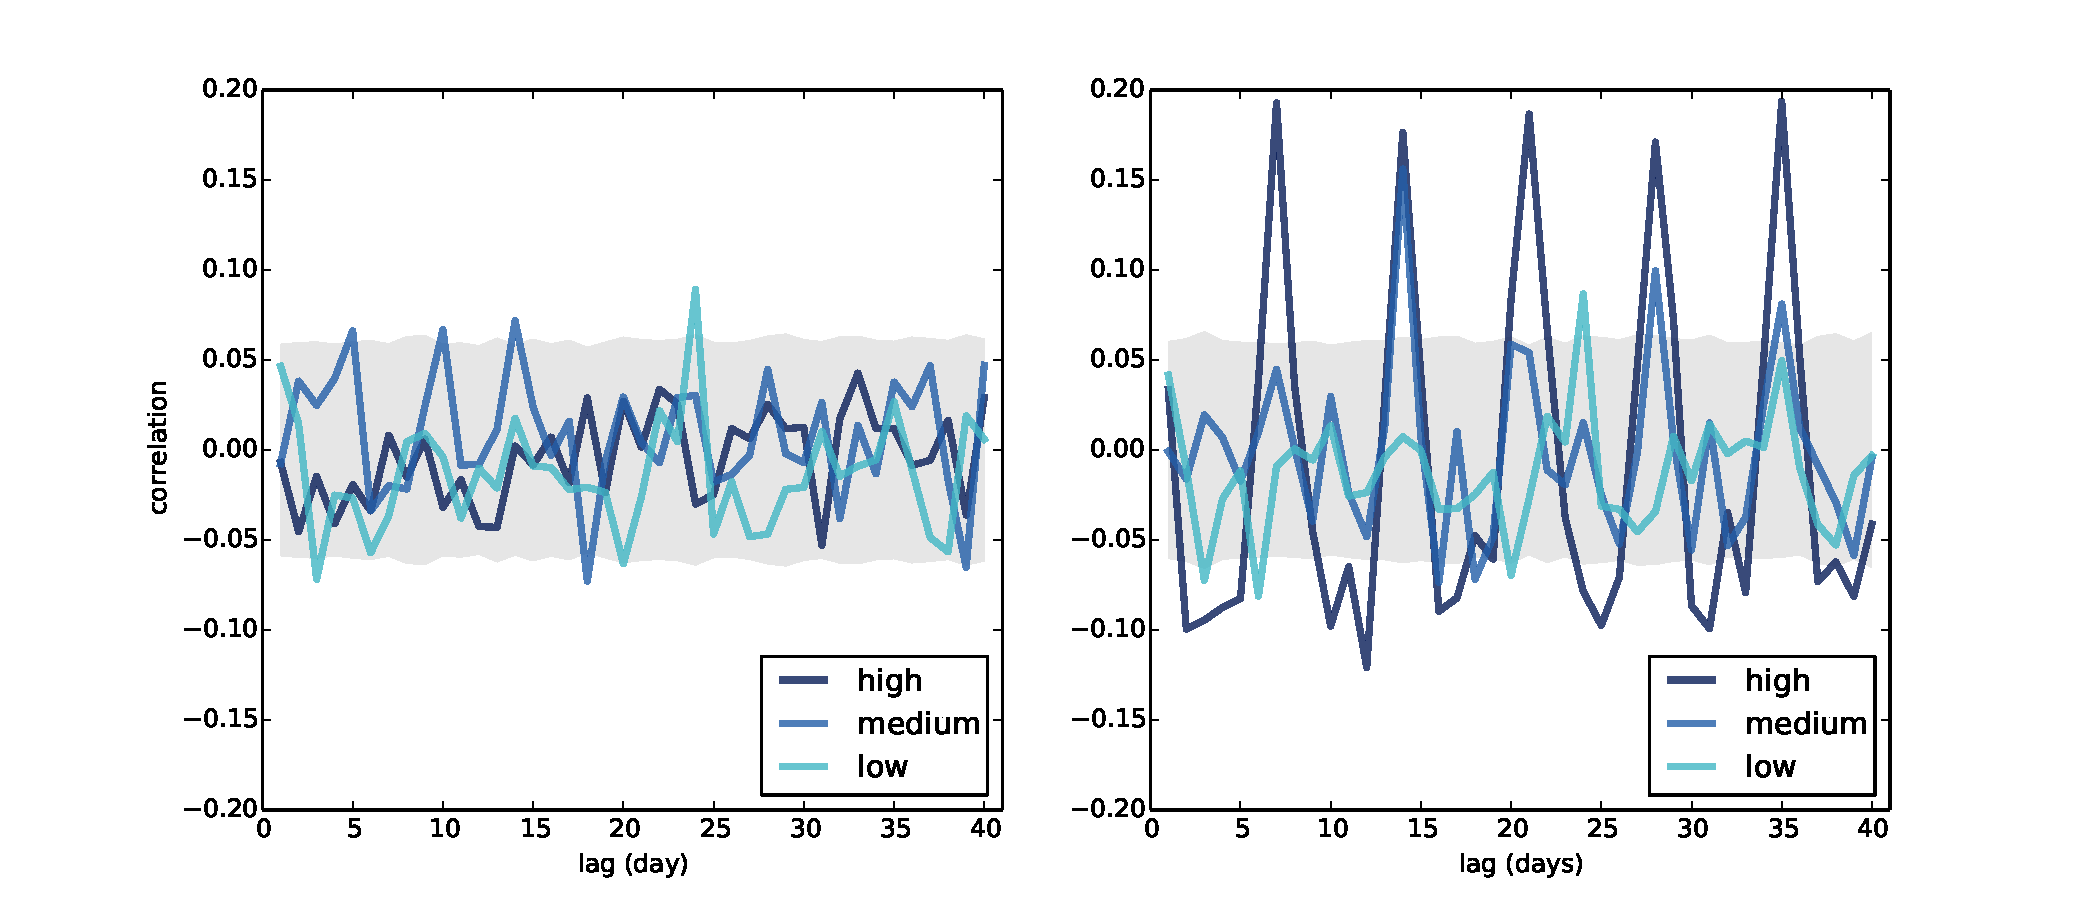
\includegraphics[height=2.5in]{figs/timeseries9.pdf}}
\caption{일별가격에 대한 자기상관 함수(좌측), 모의시험으로 주별 계절성을 갖는 일별가격에 대한 자기상관 함수(우측).}
\label{timeseries9}
\end{figure}

그림~\ref{timeseries9} (왼편)에는 {\tt nlags=40} 시차로 3개 품질 범주에 대한 자기상관함수를 보여준다.
회색지역에는 만약 실제 자기상관이 없다면 예상되는 정규 변동성이 나타나 있다; 이 범위 밖에 있는 어느 것이나 p-값이 5\%보다 작아서 통계적 유의성이 있다. 거짓양성(false positive)가 5\% 이고 120개 상관(3개 시계열에 대해서 시차 40)을 계산하기 때문에, 이 구역 박에 약 6개 점이 예상된다.
사실 7개 점이 있다. 이들 시계열에는 우연으로 설명될 수 없는 자기상관이 없다고 결론낸다.
\index{p-값 (p-value)}
  \index{유의성 (significant)} 
  \index{통계적 유의성 (statistically significant)}
\index{거짓양성 (false positive)}

잔차를 재표본추출해서 회식 지역을 계산했다. 코드는 {\tt timeseries.py} 파일에 있다; 함수는 {\tt SimulateAutocorrelation}다.
\index{재표본추출 (resampling)}

계절적 성분이 있을 때, 자기상관 함수가 어떤 느낌인지 살펴보기 위해서, 주별 주기를 더해서 모의 시험 데이터를 생성했다. 대마초 수요가 주말에 더 높다고 가정하면, 가격이 더 높을 것으로 예상할 수 있다. 효과를 모의 시험하기 위해서, 금요일 혹은 토요일 날짜를 선택하고, 가격에 \$0 에서 \$2 까지 균등분포에서 추출한 임의 금액을 더한다.
\index{모의시험 (simulation)}
\index{균등 분포 (uniform distribution)}
\index{분포 (distribution)!균등 (uniform)}

\begin{verbatim}
def AddWeeklySeasonality(daily):
    frisat = (daily.index.dayofweek==4) | (daily.index.dayofweek==5)
    fake = daily.copy()
    fake.ppg[frisat] += np.random.uniform(0, 2, frisat.sum())
    return fake
\end{verbatim}

{\tt frisat}는 부울 시리즈로, 만약 여일이 금요일 혹은 토요일이면, {\tt 참(True)}이다. {\tt fake}는 새 데이터프레임으로 원래 {\tt daily} 복사본으로 {\tt ppg}에 확률값(random value)을 더해서 변경한다. {\tt frisat.sum()}은 금요일과 토요일 전체 갯수로 생성해야하는 확률값 갯수가 된다.
\index{데이터프레임 (DataFrame)}
\index{시리즈 (Series)}
\index{부울 (boolean)}


그림~\ref{timeseries9} (오른편)에는 모의시험 계절성을 갖는 가격에 대한 자기상관 함수가 나타나 있다. 예상했듯이, 시차가 7의 곱이 될 때 가장 높다. 고급과 중급 품질에 대해 신규 상관이 통계적 유의성이 있다. 저급 품질에 대서는 유의적이지 않은데 이유는 이 범주에 잔차가 크기 때문이다; 잡음을 뚫고 보여지기 위해서는 효과가 더 커야한다.
\index{유의성 (significant)} \index{통계적 유의성 (statistically significant)}
\index{잔차 (residuals)}
\index{시차 (lag)}


\section{예측 (Prediction)}  

시계열 분석은 시간에 변화하는 시스템 행동을 조사하고 때때로 설명하는데 사용될 수 있다. 또한 예측도 할 수 있다.
\index{예측 (prediction)}

~\ref{timeregress}절에서 사용한 선형회귀는 예측에 사용될 수 있다.
RegressionResults 클래스에 {\tt predict}를 사용해서
설명변수를 포함하는 데이터프레임을 인자로 받아 예측 시퀀스를 반환한다.
다음에 코드가 있다.
\index{설명변수 (explanatory variable)}
\index{선형회귀 (linear regression)}

\begin{verbatim}
def GenerateSimplePrediction(results, years):
    n = len(years)
    inter = np.ones(n)
    d = dict(Intercept=inter, years=years)
    predict_df = pandas.DataFrame(d)
    predict = results.predict(predict_df)
    return predict
\end{verbatim}

{\tt results}는 RegressionResults 객체다; 
{\tt years}는 예측하려는 시간 값 시퀀스다.
함수가 데이터프레임을 생성하고 {\tt predict}에 전달하고 결과를 반환한다.
\index{판다스 (pandas)}
\index{데이터프레임 (DataFrame)}

만약 원하는 모든 것이, 하나의 최선을 다한 예측이라면, 완료했다.
하지만, 대부분 목적에 대해서, 오차를 정량화하는 것이 중요하다.
다른 말로, 예측이 얼마의 정확성이 있는지 알고싶다.

고려해야 하는 오류 원천이 3가지 있다.

\begin{itemize}

\item 표집오차 (Sampling error): 
예측은 추정 모수에 기반하는데, 추정 모수는 표본 확률변동에 의존한다.
만약 실험을 다시 실시한다면, 추정값이 변화할 것으로 예상된다.
\index{표집오차 (sampling error)}
\index{모수 (parameter)}

\item 확률변동 (Random variation):
설사 추정 모수가 완벽할지라도, 관측 데이터는 장기추세주변에서 확률적으로 변동하고 이러한 변동은 미래에도 계속될 것으로 예상된다.
\index{잡음 (noise)}

\item 모형화 오차 (Modeling error): 
장기 추세가 선형이 아니라는 증거를 이미 봤다. 그래서 선형 모형에 기반한 예측은 결국 실패할 것이다.
\index{모형화 오차 (modeling error)}

\end{itemize}

고려할 또 다른 오류 원천은 예상치 못한 미래 사건이다. 
농산물 가격은 날씨에 영향을 받고, 모든 가격은 정치와 법에 영향하에 있다. 이 책을 집필하고 있을 때, 대마초는 미국 두주에서 합법이고, 의료목적으로 20개 이상 주에서 합법이다. 만약 더 많은 주가 합법화한다면, 가격은 내려갈 것이다. 하지만, 연방정부가 단속한다면, 가격이 치솟을지 모른다.

모형화 오차 (modeling error)와 예상치 못한 미래 사건은 정량화하기 어렵니다. 표집오차와 확률변동은 다루기 더 쉽다. 그래서 먼저 이것을 다뤄보자.

표집오차를 정량화하기 위해서, ~\ref{regest}절에서 했던 것처럼 재표본추출법을 사용한다. 늘 그렇듯이, 목적은 만약 실험을 다시 실행한다면 무엇이 발생할 것인지 모의 시험하는데 실제 관측점을 사용하는 것이다.
모의시험은 추정 모수가 맞지만 확률 잔차가 다를 수 있다는 가정에 기반한다.
여기 모의 시험을 수행하는 함수가 있다.
\index{재표본추출 (resampling)}

\begin{verbatim}
def SimulateResults(daily, iters=101):
    model, results = RunLinearModel(daily)
    fake = daily.copy()
    
    result_seq = []
    for i in range(iters):
        fake.ppg = results.fittedvalues + Resample(results.resid)
        _, fake_results = RunLinearModel(fake)
        result_seq.append(fake_results)

    return result_seq
\end{verbatim}

{\tt daily}는 관측 가격을 포함하는 데이터프레임이다;
{\tt iters}는 모의 시험할 횟수다.
\index{데이터프레임 (DataFrame)}
\index{가격 (price)}

{\tt SimulateResults}는 ~\ref{timeregress}절로부터 {\tt RunLinearModel}을 사용해서 관측값의 기울기와 절편을 추정한다.

루프를 반복할 때마다, 잔차를 재표본추출하고 적합값에 더해서 ``fake'' 데이터셋을 생성한다. 그리고 나서, ``fake'' 데이터에 선형모형을 실행하고 RegressionResults 객체에 저장한다.
\index{모형 (model)}
\index{잔차 (residuals)}

다음 단계로 예측을 생성하는데 모의 시험 결과를 사용한다.

\begin{verbatim}
def GeneratePredictions(result_seq, years, add_resid=False):
    n = len(years)
    d = dict(Intercept=np.ones(n), years=years, years2=years**2)
    predict_df = pandas.DataFrame(d)
    
    predict_seq = []
    for fake_results in result_seq:
        predict = fake_results.predict(predict_df)
        if add_resid:
            predict += thinkstats2.Resample(fake_results.resid, n)
        predict_seq.append(predict)

    return predict_seq
\end{verbatim}

{\tt GeneratePredictions}는 이전 단계에서 결과 시퀀스 뿐만 아니라 
예측을 생성할 구간을 명시하는 부동소수점 시퀀스 {\tt years}, 그리고 재표본추출 잔차가 직선 예측에 추가해야 하는지를 말지를 나타내는 \verb"add_resid"을 인자로 받는다.
{\tt GeneratePredictions}은 RegressionResults 시퀀스를 반복해서 예측 시퀀스를 생성한다.
\index{재표본추출 (resampling)}

\begin{figure}
% timeseries.py
\centerline{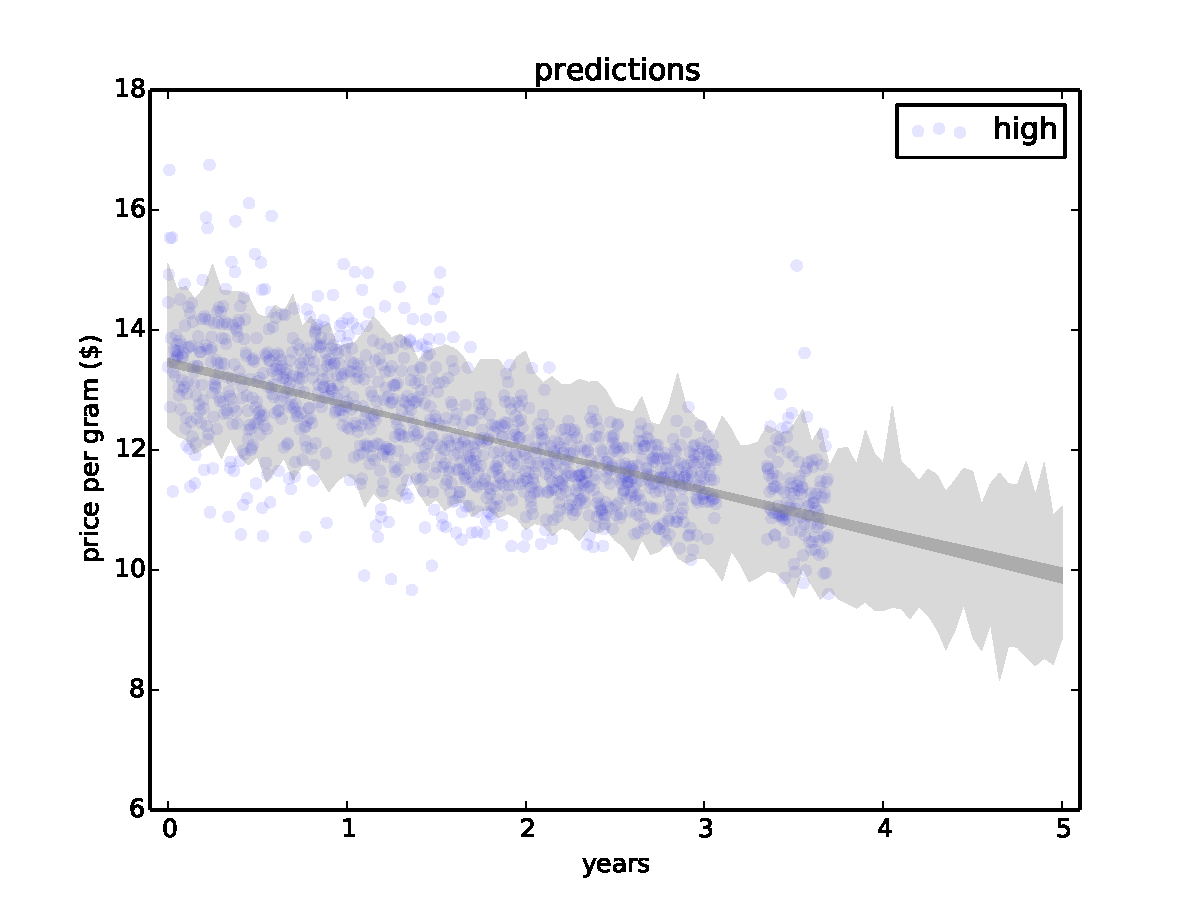
\includegraphics[height=2.5in]{figs/timeseries4.pdf}}
\caption{선형적합에 기초한 예측, 표집오차와 예측 오차에 기인한 변동성을 나타냄.}
\label{timeseries4}
\end{figure}

마지막으로, 다음에 예측으로 90\% 신뢰구간을 플롯으로 그리는 코드가 있다.
\index{신뢰구간 (confidence interval)}

\begin{verbatim}
def PlotPredictions(daily, years, iters=101, percent=90):
    result_seq = SimulateResults(daily, iters=iters)
    p = (100 - percent) / 2
    percents = p, 100-p

    predict_seq = GeneratePredictions(result_seq, years, True)
    low, high = thinkstats2.PercentileRows(predict_seq, percents)
    thinkplot.FillBetween(years, low, high, alpha=0.3, color='gray')

    predict_seq = GeneratePredictions(result_seq, years, False)
    low, high = thinkstats2.PercentileRows(predict_seq, percents)
    thinkplot.FillBetween(years, low, high, alpha=0.5, color='gray')
\end{verbatim}

{\tt PlotPredictions}이 {\tt GeneratePredictions}을 두번 호출한다; 한번은 \verb"add_resid=True"이고, 다른 한번은 \verb"add_resid=False"이다.
{\tt PercentileRows}를 사용해서 각 년도에 대해서 5번째와 95번째 백분위수를 선택한다. 그리고 나서, 경계 사이 회색지역을 플롯으로 그린다..
\index{FillBetween}

그림~\ref{timeseries4}에 결과가 나와 있다.
짙은 회색 지역이 표집오차에 대한 90\% 신뢰구간을 나타낸다; 즉,
표집때문에 추정 기울기와 절편에 대한 불확실성.
\index{표집오차 (sampling error)}

밝은 지역은 예측 오차에 대한 90\% 신뢰구간을 보여주는데,
표집오차와 확률변동 합이다.
\index{잡음 (noise)}

이들 지역이 표집오차, 확률변동을 정량화하지만, 모형화 오류는 정량화하지 않는다. 일반적으로 모형화 오류는 정량화하기 어렵다. 하지만, 이경우에 최소한 오차 원천 하나(예측치 못한 외부 사건)는 다룰 수 있다.
\index{모형화 오차 (modeling error)}

회귀 모형은 시스템이 정상성(stationary, 시불변)이 있다는 가정에 기반한다; 즉, 모형 모수는 시간에 따라 변하지 않는다.
좀더 구체적으로, 기울기와 절편 뿐만 아니라 잔차 분포도 일정하다고 가정한다.
\index{정상성 모형 (stationary model)}
\index{모수 (parameter)}

하지만, 그림~\ref{timeseries10}에 있는 이동 평균을 살펴보면, 최소한 관측 기간동안 한번 기울기는 변하고 잔차 분산이 후반부보다 전반부에서 더 큰 것처럼 보인다.
\index{기울기 (slope)}

결과로, 추정한 모수는 관측 기간에 의존성이 있다.
이것이 예측에 얼마나 많은 효과를 갖는지 살펴보기 위해서,
다른 시작과 종료 날짜를 갖는 관측 구간을 사용하도록 {\tt SimulateResults}를 연장한다.
구현은 {\tt timeseries.py} 파일에 있다.
\index{모의시험 (simulation)}

\begin{figure}
% timeseries.py
\centerline{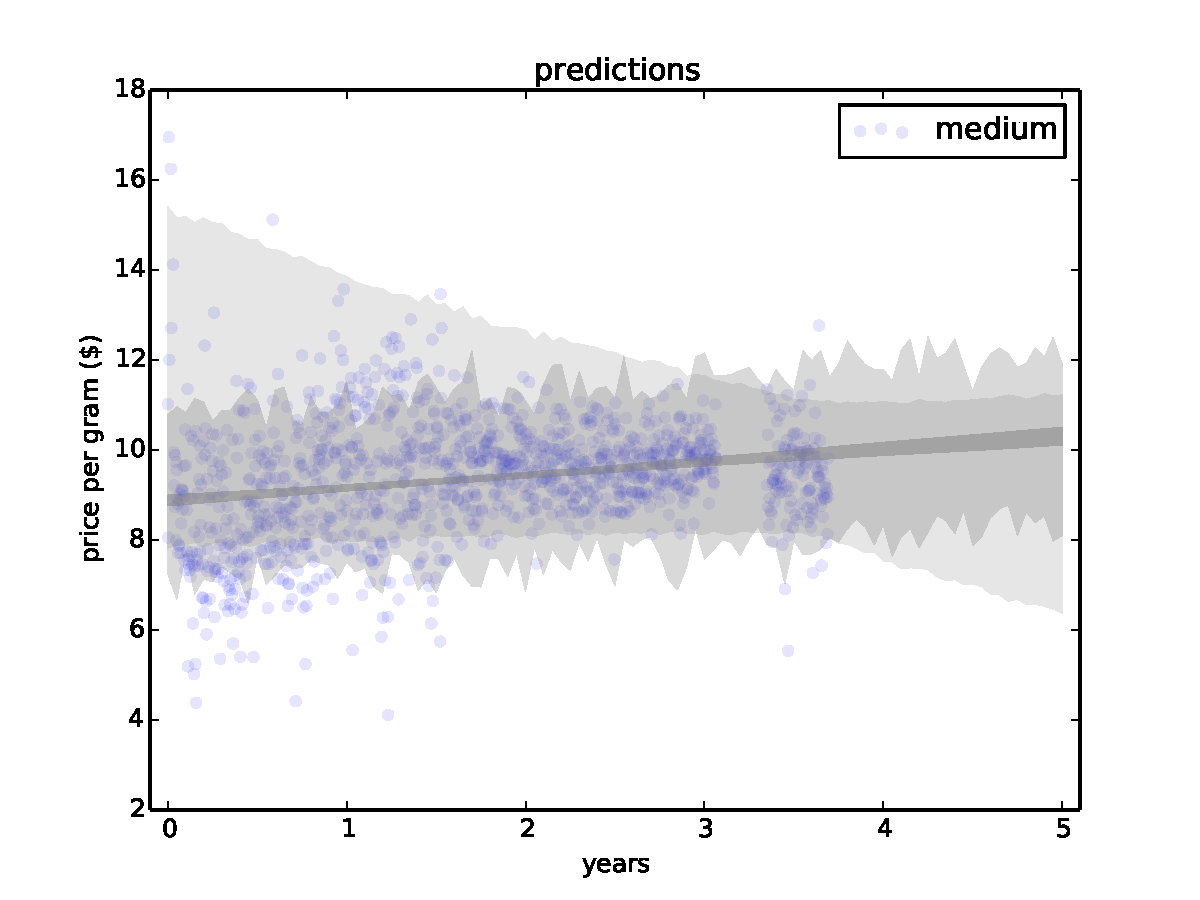
\includegraphics[height=2.5in]{figs/timeseries5.pdf}}
\caption{선형적합에 기초한 예측, 관측점 간격에 기인한 변동성을 나타냄.}
\label{timeseries5}
\end{figure}

그림~\ref{timeseries5}에 중간 품질 대마초에 대한 결과가 나와 있다.
옅은 회색 구역이 신뢰구간을 보여주는데 표집오차, 확률변동, 관측구간 변동으로 인한 불확실성이 포함한다.
\index{신뢰구간 (confidence interval)}
\index{구간 (interval)}

전체 구간에 기반한 모형이 양수 기울기를 갖고 있는데, 가격이 오르고 있다는 것을 나타낸다. 하지만, 가장 최신 구간은 하락하는 가격 신호를 보여준다. 
그래서 가장 최신 데이터에 기반한 모형은 음수 기울기를 갖는다.
결과로, 가장 폭이 넗은 구간은 내년에 하락하는 가격 가능성을 포함한다.
\index{모형 (model)}


\section{추가 읽기}
시계열 분석은 큰 주제다; 이번 장에서 단지 표면만 긁었을 뿐이다.
시계열 데이터로 작업하는데 중요한 도구는 자기회귀로 여기서는 다루지 않았다. 왜냐하면, 작업한 예제 데이터에 사용하기에 적합하지 않았기 때문이다.
\index{시계열 (time series)}

하지만, 이장에 있는 내용를 학습하면, 자기회귀를 학습할 준비가 된 것이다. 추천하는 한 교재는 Philipp Janert가 저술한 책, {\it Data Analysis with Open Source Tools} O'Reilly Media, 2011. 
시계열에 대한 장에서 여기서 다루지 않는 내용을 학습할 수 있다.
\index{Janert, Philipp}


\section{연습문제}

이 연습문제에 대한 저자 해답은 \verb"chap12soln.py"에 나와있다.

\begin{exercise}
이번 장에서 저자가 사용한 선형모형은 선형이라는 명백한 결점이 있고,
가격이 시간에 따라 선형으로 변할 것이라고 예측할 이유는 없다.
\ref{nonlinear}~절에서 했던 것처럼, 2차항을 추가해서 모형에 유연성을 더할 수 있다.

\index{비선형}
\index{선형 모형}
\index{2차 모형}

2차 모형을 사용해서 시계열 일별가격을 적합할 수 있고,
모형을 사용해서 예측값도 생성할 수 있다.
2차 모형을 돌리는 {\tt RunLinearModel} 버젼을 작성해야할 것이다.
하지만, 예측을 생성하는데 {\tt timeseries.py}에 나온 코드를 재사용할 수도 있다.

\index{예측}

\end{exercise}

\begin{exercise}

\ref{hypotest}~절에 나온 {\tt HypothesisTest}을 확장하는 
클래스를 정의하는데 명칭은 {\tt SerialCorrelationTest}이다.
데이터로 시계열과 시차(lag)를 받아서, 주어진 시차를 갖는 
시계열 데이터의 계열상관을 계산하고 나서,
관측된 상관에 대한 p-값을 계산한다.

\index{HypothesisTest}
\index{p-값}
\index{시차}

이 클래스를 사용해서 원가격 데이터에 나온 계열 상관이 통계적으로 유의적인지 검정한다.
또한, 선형모형과 (만약 이전 예제를 수행했다면) 2차 모형의 잔차를 검정한다.
\index{2차 모형}
  \index{유의적인} \index{통계적으로 유의한}

\end{exercise}

\begin{exercise}
예측을 만들어 내는데, EWMA 모형을 확장하는 몇가지 방식이 있다.
가장 단순한 방법중의 하나는 다음과 같다:
\index{EWMA}

\begin{enumerate}

\item 시계열 EWMA를 계산하고, 가장 마지막 점을 절편 {\tt inter}으로 사용한다.

\item 시계열의 연속 요소사이에 EWMA 차이를 계산하고, 가장 마지막 점을 기울기 {\tt slope}로 사용한다.
\index{기울기}

\item 미래 시점에 값을 예측하는데, {\tt inter + slope * dt}을 계산한다.
여기서 {\tt dt}는 예측 시점과 가장 마지막 예측 시점의 차이다.
\index{예측}

\end{enumerate}

이 방법을 사용해서, 마지막 관측점 다음 연도에 대한 예측을 생성한다.
몇가지 힌드는 다음과 같다:

\begin{itemize}

\item {\tt timeseries.FillMissing}을 사용해서 분석을 돌리기 전에 결측값을 채워넣는다.
이런 방식으로 연속된 요소값 사이 시점이 일치한다.
\index{결측값}

\item {\tt Series.diff}을 사용해서 연속된 요소 사이 차이를 계산한다.
\index{시리즈}

\item {\tt reindex}을 사용해서 데이터프레임을 미래로 연장한다.
\index{reindex}

\item {\tt fillna}을 사용해서 예측한 값을 데이터프레임에 넣는다.
\index{fillna}

\end{itemize}

\end{exercise}


\section{용어 사전}

\begin{itemize}

\item 시계열(time series): 각 값이 시간도장(timestamp)과 연관된 데이터셋. 종종 측정값과 추집된 시점 계열.
\index{시계열 (time series)}

\item 윈도우 (window): 이동 평균을 계산하는 종종 사용되는 시계열에 연속값 시퀀스.
\index{윈도우 (window)}

\item 이동평균 (moving average): 겹쳐지지 않는 일련의 윈도우에 대한 평균을 계산함으로써 시계열에 잠재하는 추세를 추정하는데 사용되는 여러 통계량 중의 하나.
\index{이동평균 (moving average)}

\item 이동평균 (rolling mean):각 윈도우 평균값에 기반한 이동평균.
\index{이동평균 (rolling mean)}

\item 지수가중이동평균 (exponentially-weighted moving average, EWMA): 
가중평균에 기반한 이동평균으로 가장 최근 값에 가장 높은 가중치를 두고, 이전 값에 대해서는 지수적으로 줄어드는 가중치를 둔다.
\index{지수가중이동평균 (exponentially-weighted moving average)}
\index{EWMA}

\item 스팬 (span): 가중치가 얼마나 빨리 줄어드는지를 결정하는 EWMA 모수.
\index{스팬 (span)}

\item 계열상관 (serial correlation): 
한 시계열과 이동된 혹은 시차이동한 자신 시계열과 상관.
\index{계열상관 (serial correlation)}

\item 시차 (lag): 계열 상관 혹은 자기상관에서 이동 크기.
\index{시차 (lag)}

\item 자기상관 (autocorrelation): 임의 시차를 갖는 계열상관에 대한 좀더 일반적인 용어.
\index{자기상관 함수 (autocorrelation function)}

\item 자기상관 함수 (autocorrelation function): 
시차에서 계열상관으로 매핑하는 함수.

\item 정상성 (stationary): 만약 모수와 잔차 분포가 시간에 따라 변화하지 않는다면, 모형이 정상성이 있다.
\index{모형 (model)}
\index{정상성 모형 (stationary model)}

\end{itemize}

